% Source: Code/ML_overlay/ir_rgb_registration/paper/ml_overlay_report_materials/ir_rgb_registration_report/figures/fig_raft_architecture.tex
\documentclass[tikz,border=10pt]{standalone}
\usepackage{tikz}
\usepackage{amsfonts}
\usetikzlibrary{positioning,shapes.geometric,arrows.meta,calc,decorations.pathmorphing}

\definecolor{Garnet}{RGB}{115,0,10}
\definecolor{Rose}{RGB}{204,46,64}
\definecolor{Atlantic}{RGB}{70,106,159}
\definecolor{Congaree}{RGB}{31,65,77}
\definecolor{Horseshoe}{RGB}{101,120,11}
\definecolor{Honeycomb}{RGB}{164,145,55}
\definecolor{Black90}{RGB}{54,54,54}

\begin{document}
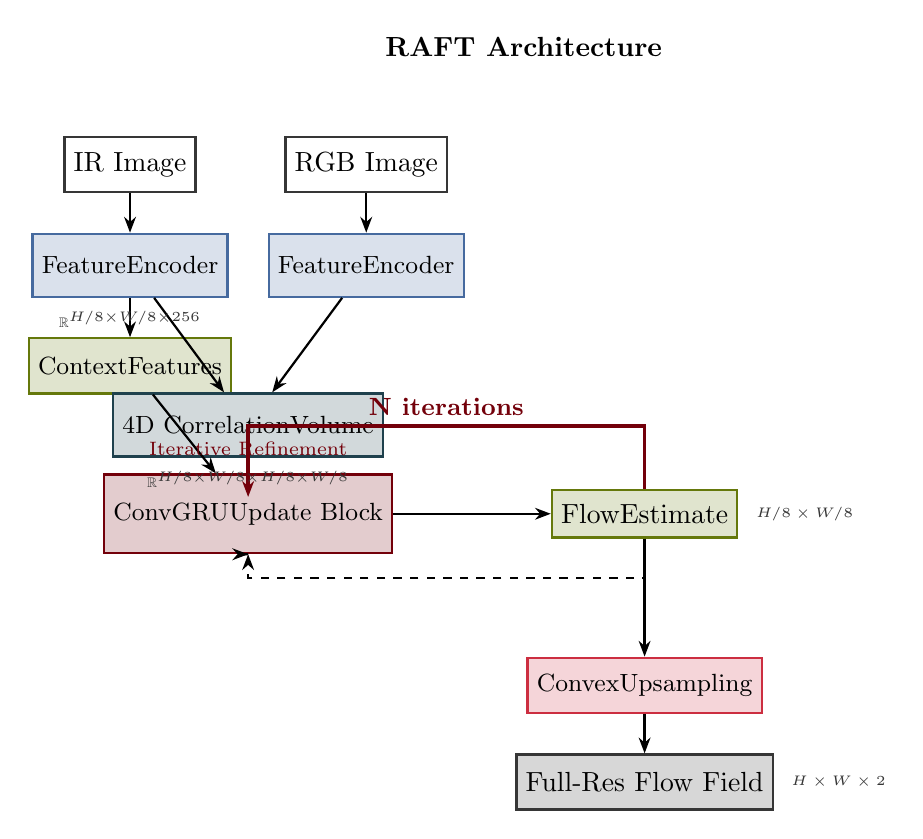
\begin{tikzpicture}[
    encoder/.style={rectangle,draw=Atlantic,fill=Atlantic!20,thick,minimum width=2cm,minimum height=0.8cm,font=\small},
    corr/.style={rectangle,draw=Congaree,fill=Congaree!20,thick,minimum width=2.5cm,minimum height=0.8cm,font=\small},
    gru/.style={rectangle,draw=Garnet,fill=Garnet!20,thick,minimum width=2cm,minimum height=1cm,font=\small},
    context/.style={rectangle,draw=Horseshoe,fill=Horseshoe!20,thick,minimum width=1.8cm,minimum height=0.7cm,font=\small},
    upsample/.style={rectangle,draw=Rose,fill=Rose!20,thick,minimum width=2cm,minimum height=0.7cm,font=\small},
    arrow/.style={-{Stealth[length=2mm]},thick}
]

\node[font=\bfseries] at (6,9) {RAFT Architecture};

% Input images
\node[rectangle,draw=Black90,thick,minimum width=1.5cm,minimum height=0.7cm] (ir-input) at (1,7.5) {IR Image};
\node[rectangle,draw=Black90,thick,minimum width=1.5cm,minimum height=0.7cm] (rgb-input) at (4,7.5) {RGB Image};

% Feature encoders
\node[encoder,below=0.5cm of ir-input] (ir-feat) {Feature\\Encoder};
\node[encoder,below=0.5cm of rgb-input] (rgb-feat) {Feature\\Encoder};

\draw[arrow] (ir-input) -- (ir-feat);
\draw[arrow] (rgb-input) -- (rgb-feat);

% Context encoder (from IR only)
\node[context,below=0.5cm of ir-feat] (context) {Context\\Features};
\draw[arrow] (ir-feat) -- (context);

% Correlation volume
\node[corr,below=1.2cm of rgb-feat,xshift=-1.5cm] (corr-vol) {4D Correlation\\Volume};
\draw[arrow] (ir-feat) -- (corr-vol);
\draw[arrow] (rgb-feat) -- (corr-vol);

% Correlation lookup
\node[rectangle,draw=Congaree,fill=Congaree!20,thick,minimum width=1.8cm,minimum height=0.7cm,below=0.5cm of corr-vol] (corr-lookup) {Correlation\\Lookup};
\draw[arrow] (corr-vol) -- (corr-lookup);

% GRU update block
\node[gru,below=1cm of context,xshift=1.5cm] (gru) {ConvGRU\\Update Block};

% Flow estimate
\node[rectangle,draw=Horseshoe,fill=Horseshoe!20,thick,minimum width=1.5cm,minimum height=0.6cm,right=2cm of gru] (flow-est) {Flow\\Estimate};

% Recurrent loop
\draw[arrow] (context) -- (gru);
\draw[arrow] (corr-lookup) -- (gru);
\draw[arrow] (gru) -- (flow-est);

% Feedback loop
\draw[arrow,Garnet,very thick] (flow-est.north) -- ++(0,0.8) -| node[pos=0.25,above,font=\small\bfseries] {N iterations} (corr-lookup.north);

% Input flow to correlation lookup
\draw[arrow,dashed] (flow-est.south) -- ++(0,-0.5) -| (corr-lookup.south);

% Convex upsampling
\node[upsample,below=1.5cm of flow-est] (upsample) {Convex\\Upsampling};
\draw[arrow] (flow-est) -- (upsample);

% Final output
\node[rectangle,draw=Black90,fill=Black90!20,thick,minimum width=2.2cm,minimum height=0.7cm,below=0.5cm of upsample] (output) {Full-Res Flow Field};
\draw[arrow] (upsample) -- (output);

% Annotations
\node[font=\tiny,text=Black90,below=0.05cm of ir-feat] {$\mathbb{R}^{H/8 \times W/8 \times 256}$};
\node[font=\tiny,text=Black90,below=0.05cm of corr-vol] {$\mathbb{R}^{H/8 \times W/8 \times H/8 \times W/8}$};
\node[font=\tiny,text=Black90,right=0.1cm of flow-est] {$H/8 \times W/8$};
\node[font=\tiny,text=Black90,right=0.1cm of output] {$H \times W \times 2$};

% Iteration annotation
\node[font=\scriptsize,text=Garnet,above=0.1cm of gru] {Iterative Refinement};

\end{tikzpicture}
\end{document}
